\documentclass{standalone}
\usepackage{tikz}
\usetikzlibrary{shapes.geometric}
\begin{document}
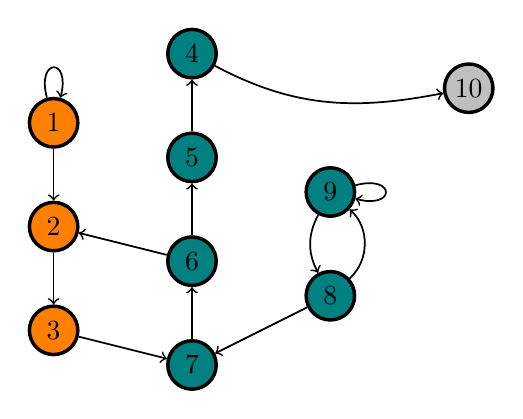
\begin{tikzpicture}
[every node/.style={inner sep=0pt}]
\node (1) [circle, minimum size=17.5pt, fill=orange, line width=1.25pt, draw=black] at (37.5pt, -37.5pt) {\textcolor{black}{1}};
\node (2) [circle, minimum size=17.5pt, fill=orange, line width=1.25pt, draw=black] at (37.5pt, -75.0pt) {\textcolor{black}{2}};
\node (3) [circle, minimum size=17.5pt, fill=orange, line width=1.25pt, draw=black] at (37.5pt, -112.5pt) {\textcolor{black}{3}};
\node (8) [circle, minimum size=17.5pt, fill=teal, line width=1.25pt, draw=black] at (137.5pt, -100.0pt) {\textcolor{black}{8}};
\node (4) [circle, minimum size=17.5pt, fill=teal, line width=1.25pt, draw=black] at (87.5pt, -12.5pt) {\textcolor{black}{4}};
\node (5) [circle, minimum size=17.5pt, fill=teal, line width=1.25pt, draw=black] at (87.5pt, -50.0pt) {\textcolor{black}{5}};
\node (6) [circle, minimum size=17.5pt, fill=teal, line width=1.25pt, draw=black] at (87.5pt, -87.5pt) {\textcolor{black}{6}};
\node (7) [circle, minimum size=17.5pt, fill=teal, line width=1.25pt, draw=black] at (87.5pt, -125.0pt) {\textcolor{black}{7}};
\node (9) [circle, minimum size=17.5pt, fill=teal, line width=1.25pt, draw=black] at (137.5pt, -62.5pt) {\textcolor{black}{9}};
\node (10) [circle, minimum size=17.5pt, fill=lightgray, line width=1.25pt, draw=black] at (187.5pt, -25.0pt) {\textcolor{black}{10}};
\draw [line width=0.625, ->, color=black, loop above] (1) to (1);
\draw [line width=0.625, ->, color=black] (1) to  (2);
\draw [line width=0.625, ->, color=black] (2) to  (3);
\draw [line width=0.625, ->, color=black] (5) to  (4);
\draw [line width=0.625, ->, color=black] (6) to  (5);
\draw [line width=0.625, ->, color=black] (7) to  (6);
\draw [line width=0.625, ->, color=black] (8) to  (7);
\draw [line width=0.625, ->, color=black] (9) to  [in=118, out=242] (8);
\draw [line width=0.625, ->, color=black] (8) to  [in=318, out=42] (9);
\draw [line width=0.625, ->, color=black, loop right] (9) to (9);
\draw [line width=0.625, ->, color=black] (4) to  [in=191, out=332] (10);
\draw [line width=0.625, ->, color=black] (6) to  (2);
\draw [line width=0.625, ->, color=black] (3) to  (7);

\end{tikzpicture}

\end{document}
